\section{}
% a) Calculate the accuracy and repeatability at each displacement of the large target. 
% (i.e., calculate the accuracy and repeatability when the target is at 100 mm, then calculate 
% them again at 200 mm, etc etc). Also, the accuracy and repeatability at each displacement 
% for the small target. Summarize the results in a table. Make two plots: i) one plot showing 
% the accuracy of the sensor (y-axis) as a function of target displacement (x-axis) for each 
% target size (i.e. two data sets are plotted on the same plot). ii) one plot showing the 
% repeatability of the sensor (y-axis) as a function of target displacement (x-axis) for each 
% target size.
\subsection{}
The accuracy and repeatability of the sensor was calculated for each displacement of the large and small target. The results are shown in Table \ref{tab:Q3a}. 


\begin{table}[h]
    \centering
    \caption{Accuracy and repeatability at each displacement of the large and small target}
    \label{tab:Q3a}
    \begin{tabular}{ccccc}
        \hline
        & \multicolumn{2}{c}{Large Target} & \multicolumn{2}{c}{Small Target} \\
        Displacement & Accuracy & Repeatability & Accuracy & Repeatability \\
        (mm) & (mm) & (mm) & (mm) & (mm) \\
        \midrule
        100 & 21 & 2 & 6 & 3 \\
        200 & 24 & 2 & 9 & 2 \\
        300 & 23 & 3 & 7 & 8 \\
        400 & 24 & 3 & 35 & 15 \\
        500 & 28 & 5 & 125 & 116 \\
        600 & 33 & 11 & 267 & 307 \\
        700 & 36 & 14 & 285 & 358 \\
        800 & 41 & 27 & 255 & 392 \\
        900 & 69 & 73 & 258 & 470 \\
        1000 & 70 & 135 & 168 & 253 \\
        \hline
    \end{tabular}
\end{table}

A sample calculation for the accuracy and repeatability of the large and small targets at 100mm is shown below. First a deviation table was created. 
The deviation table is shown in Table \ref{tab:Q3a-deviation}.

\begin{table}[h]
    \centering
    \caption{Deviation table for large and small targets at 100mm}
    \label{tab:Q3a-deviation}
    \begin{tabular}{ccc}
        \hline
        & \multicolumn{2}{c}{Deviation Reading} \\
        \cline{2-3}
        Displacement & Large & Small \\
        (mm) & (mm) & (mm) \\
        \midrule
        100 & 20 & -4 \\
        100 & 20 & -3 \\
        100 & 20 & -4 \\
        100 & 20 & -3 \\
        100 & 20 & -4 \\
        100 & 20 & -4 \\
        100 & 20 & -4 \\
        100 & 21 & -6 \\
        100 & 20 & -3 \\
        100 & 19 & -3 \\
        \hline
    \end{tabular}
\end{table}

Accuracy is the maximum deviation, while repeatability is the difference between the maximum and minimum deviation.

\[
    \boxed{\text{Accuracy}_\text{large} = \max(\text{Deviation}_\text{large}) = 21 \text{ mm}}
\]
\[
    \boxed{\text{Repeatability}_\text{large} = \max(\text{Deviation}_\text{large}) - \min(\text{Deviation}_\text{large}) = 21 - 19 = 2 \text{ mm}}
\]

\FloatBarrier
The accuracy and repeatability of the sensor was plotted as a function of target displacement for each target size. The results are shown in Fig. \ref{fig:Q3acc} 
and Fig. \ref{fig:Q3rep} respectively.
\begin{figure}[h]
    \centering
    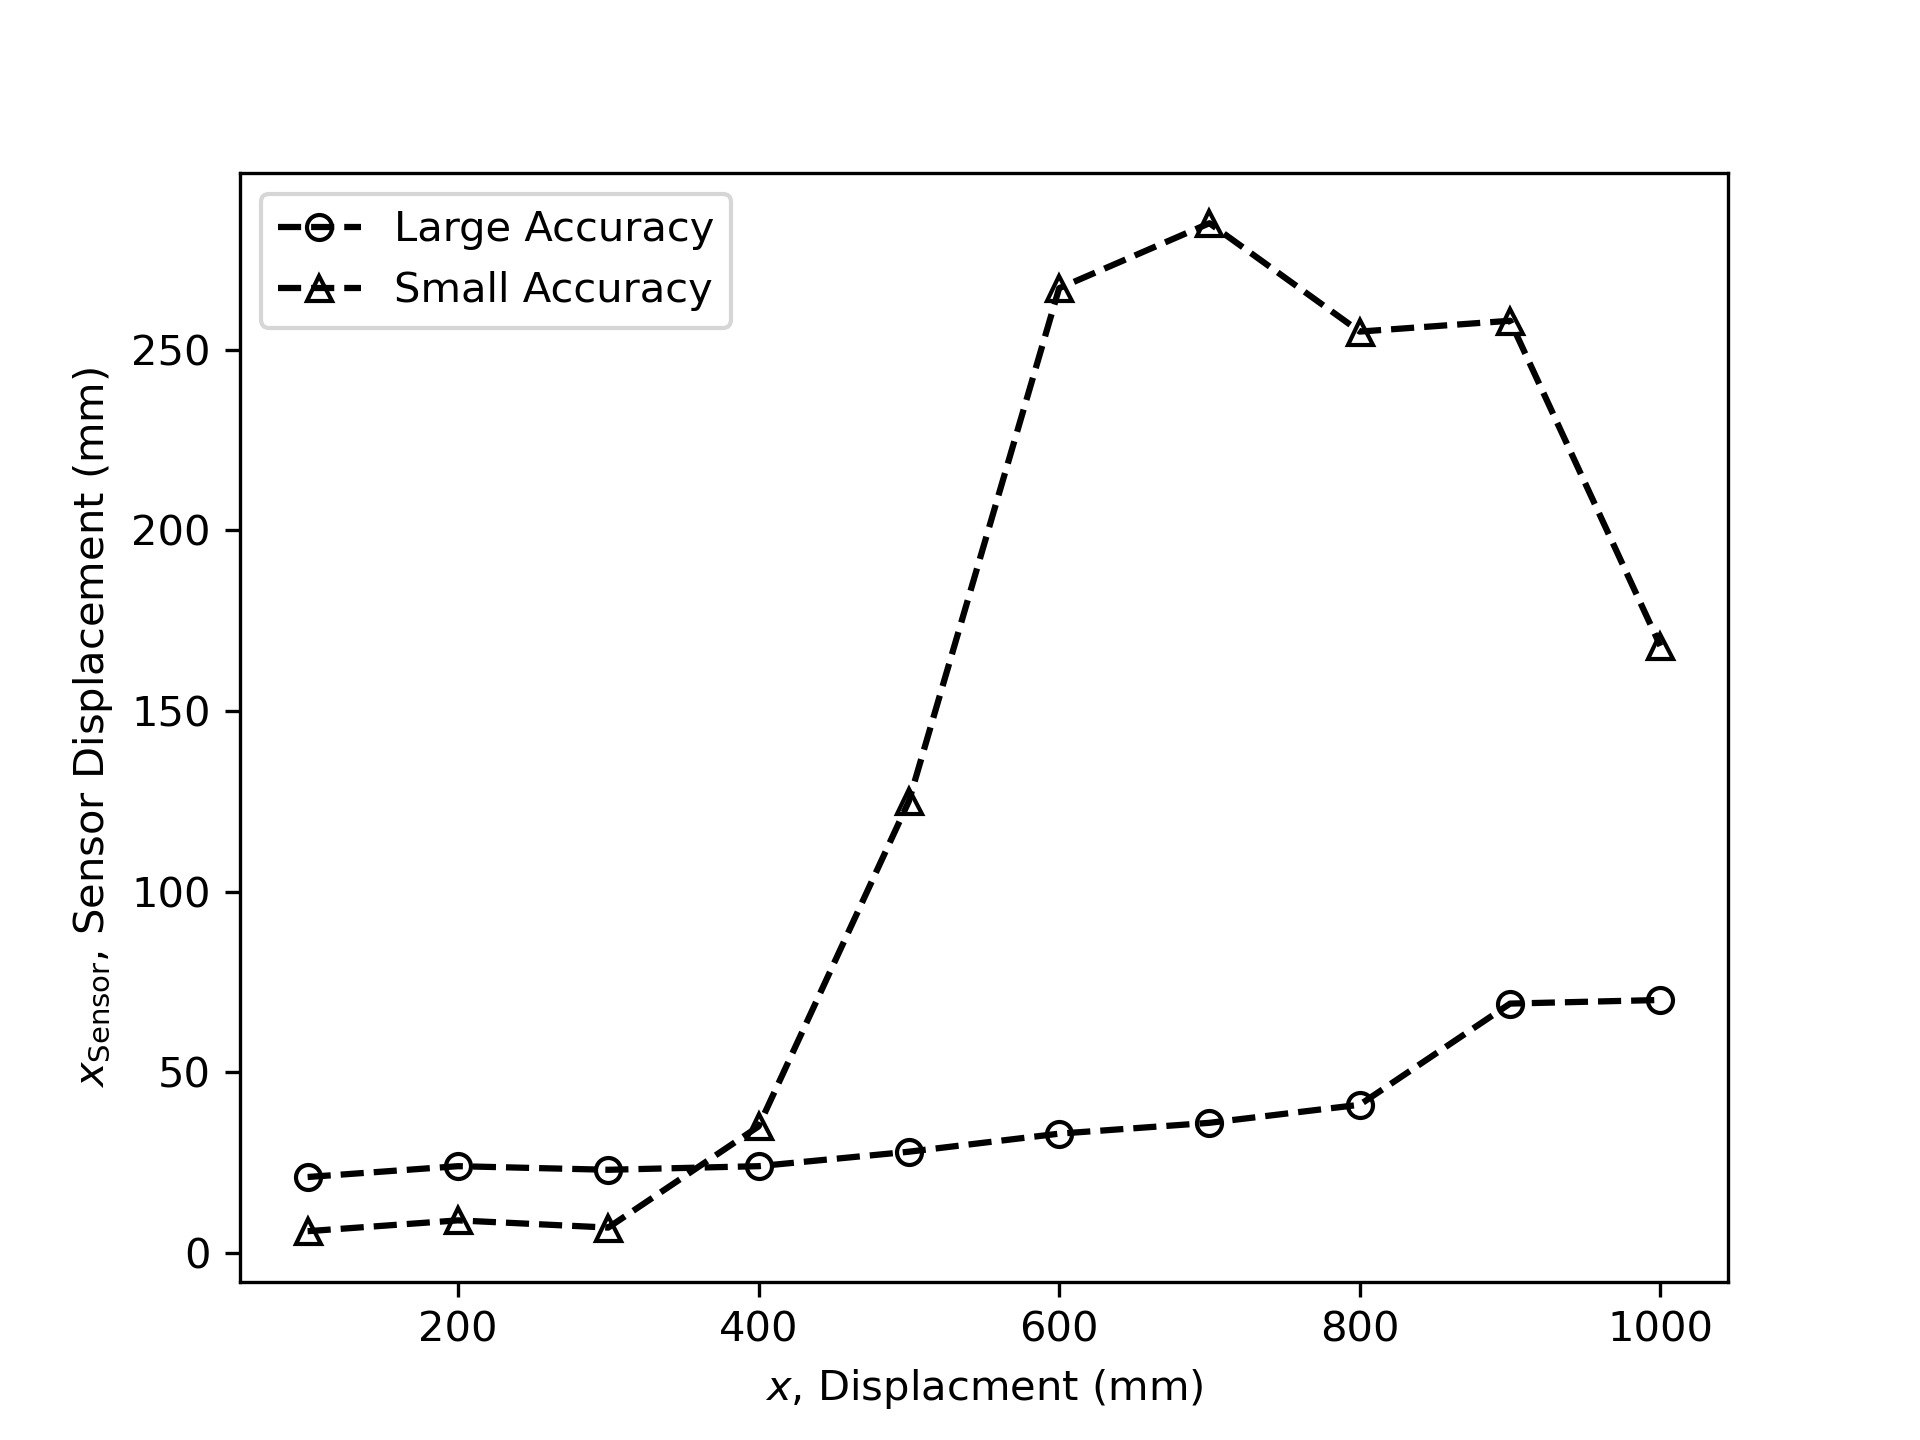
\includegraphics[width=0.6\linewidth]{matplotlib/Q3acc.png}
    \caption{Accuracy of the sensor as a function of target displacement for each target size}
    \label{fig:Q3acc}
\end{figure}

\begin{figure}[h]
    \centering
    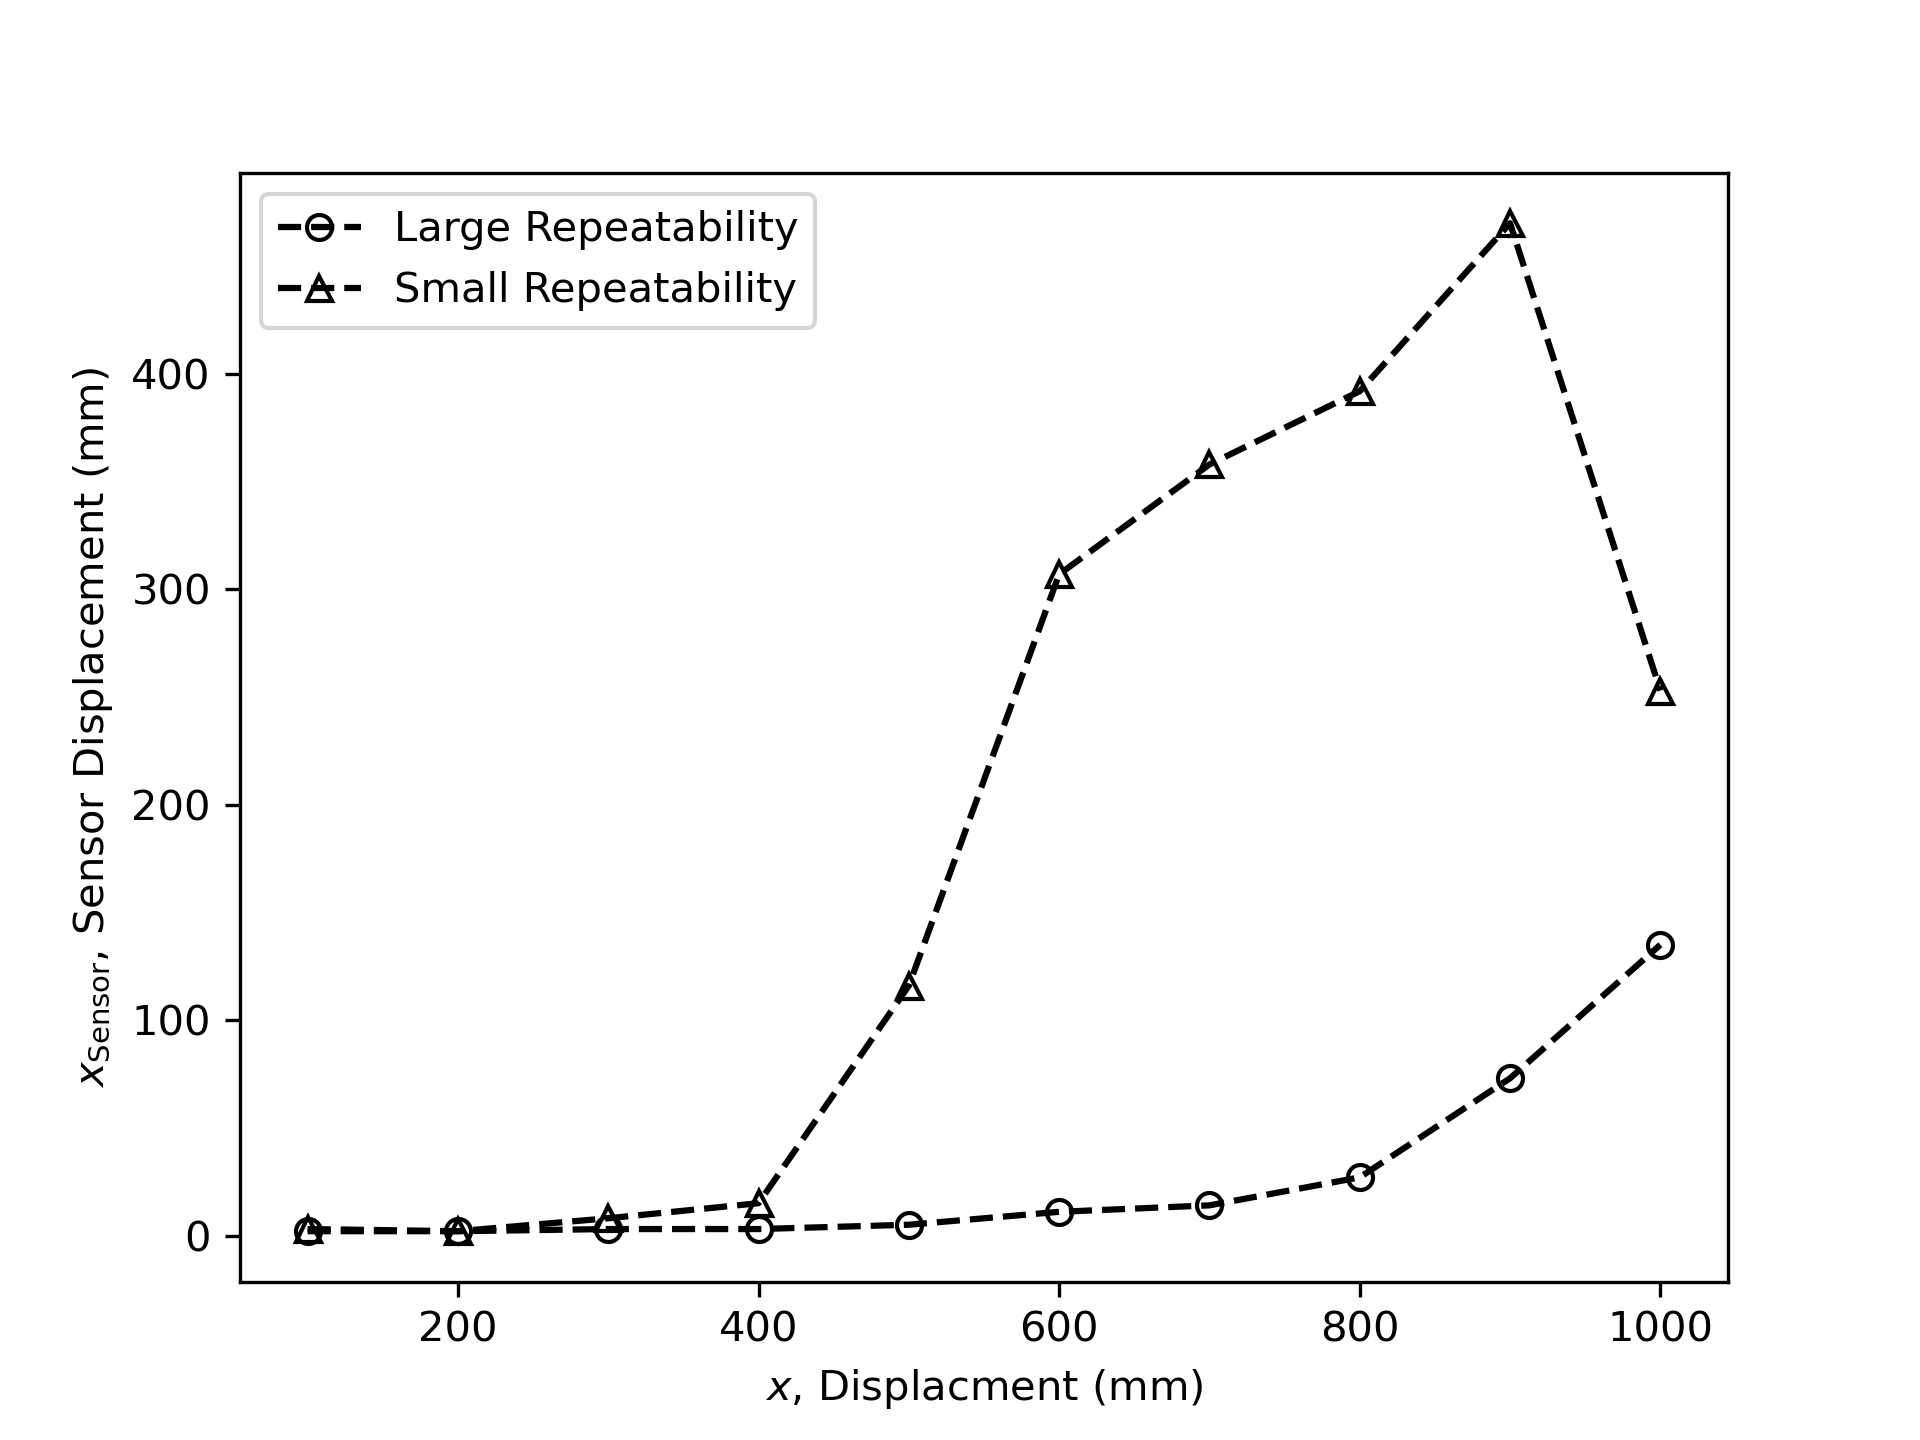
\includegraphics[width=0.6\linewidth]{matplotlib/Q3rep.png}
    \caption{Repeatability of the sensor as a function of target displacement for each target size}
    \label{fig:Q3rep}
\end{figure}

\FloatBarrier
\subsection{}
% b) How does the accuracy of the sensor change with target size? Why?

The accuracy of the sensor increases with target size and decreases with target displacement. This is because the larger target has a 
bigger surface area, so more light is reflected back to the sensor. 

Observing the target signal strengths, the large target had a higher signal strength than the small target for a given displacement. Status 2 was reached
at a lower displacement for the smaller target than the larger target, meaning the sensor had less confidence in the reading provided.

In Fig. \ref{fig:Q3acc}, the accuracy of the smaller target was slightly higher than the larger target at 100mm, 200mm, and 300mm. This diverges
quickly as the displacement increases.  